\section{Additional Results}
\label{app:additional_results}

%% =============================================================================
\subsection{Overall Performance Results}
\label{app:overall_results}

\begin{table}[htbp]
\centering
\caption{Overall model performance on GPSBench (\% accuracy).}
\label{tab:main_results_overall}
\begin{tabular}{lcc}
\toprule
\textbf{Model} & \textbf{Applied} & \textbf{Pure GPS} \\
\midrule
GPT-5.1 & 72.0 & \textbf{84.4} \\
GPT-5-mini & \textbf{74.1} & 73.0 \\
GPT-5-nano & 63.5 & 55.2 \\
GPT-4.1 & 73.3 & 60.9 \\
GPT-4.1-mini & 70.5 & 56.6 \\
\midrule
Gemini-2.5-Pro & 71.7 & 76.7 \\
Gemini-2.5-Flash & 73.4 & 58.5 \\
\midrule
Claude-Haiku-4.5 & 71.9 & 54.7 \\
\midrule
Mistral-Large & 72.5 & 54.3 \\
Mistral-Small-24B & 59.8 & 42.1 \\
\midrule
Qwen3-235B & 69.8 & 55.2 \\
Qwen3-30B & 53.9 & 53.1 \\
Qwen3-14B & 50.3 & 35.4 \\
Qwen3-8B & 47.1 & 33.3 \\
\bottomrule
\end{tabular}
\end{table}

%% =============================================================================
\subsection{Per-Task Performance Breakdown}
\label{app:per_task}

\begin{figure*}[htbp]
\centering
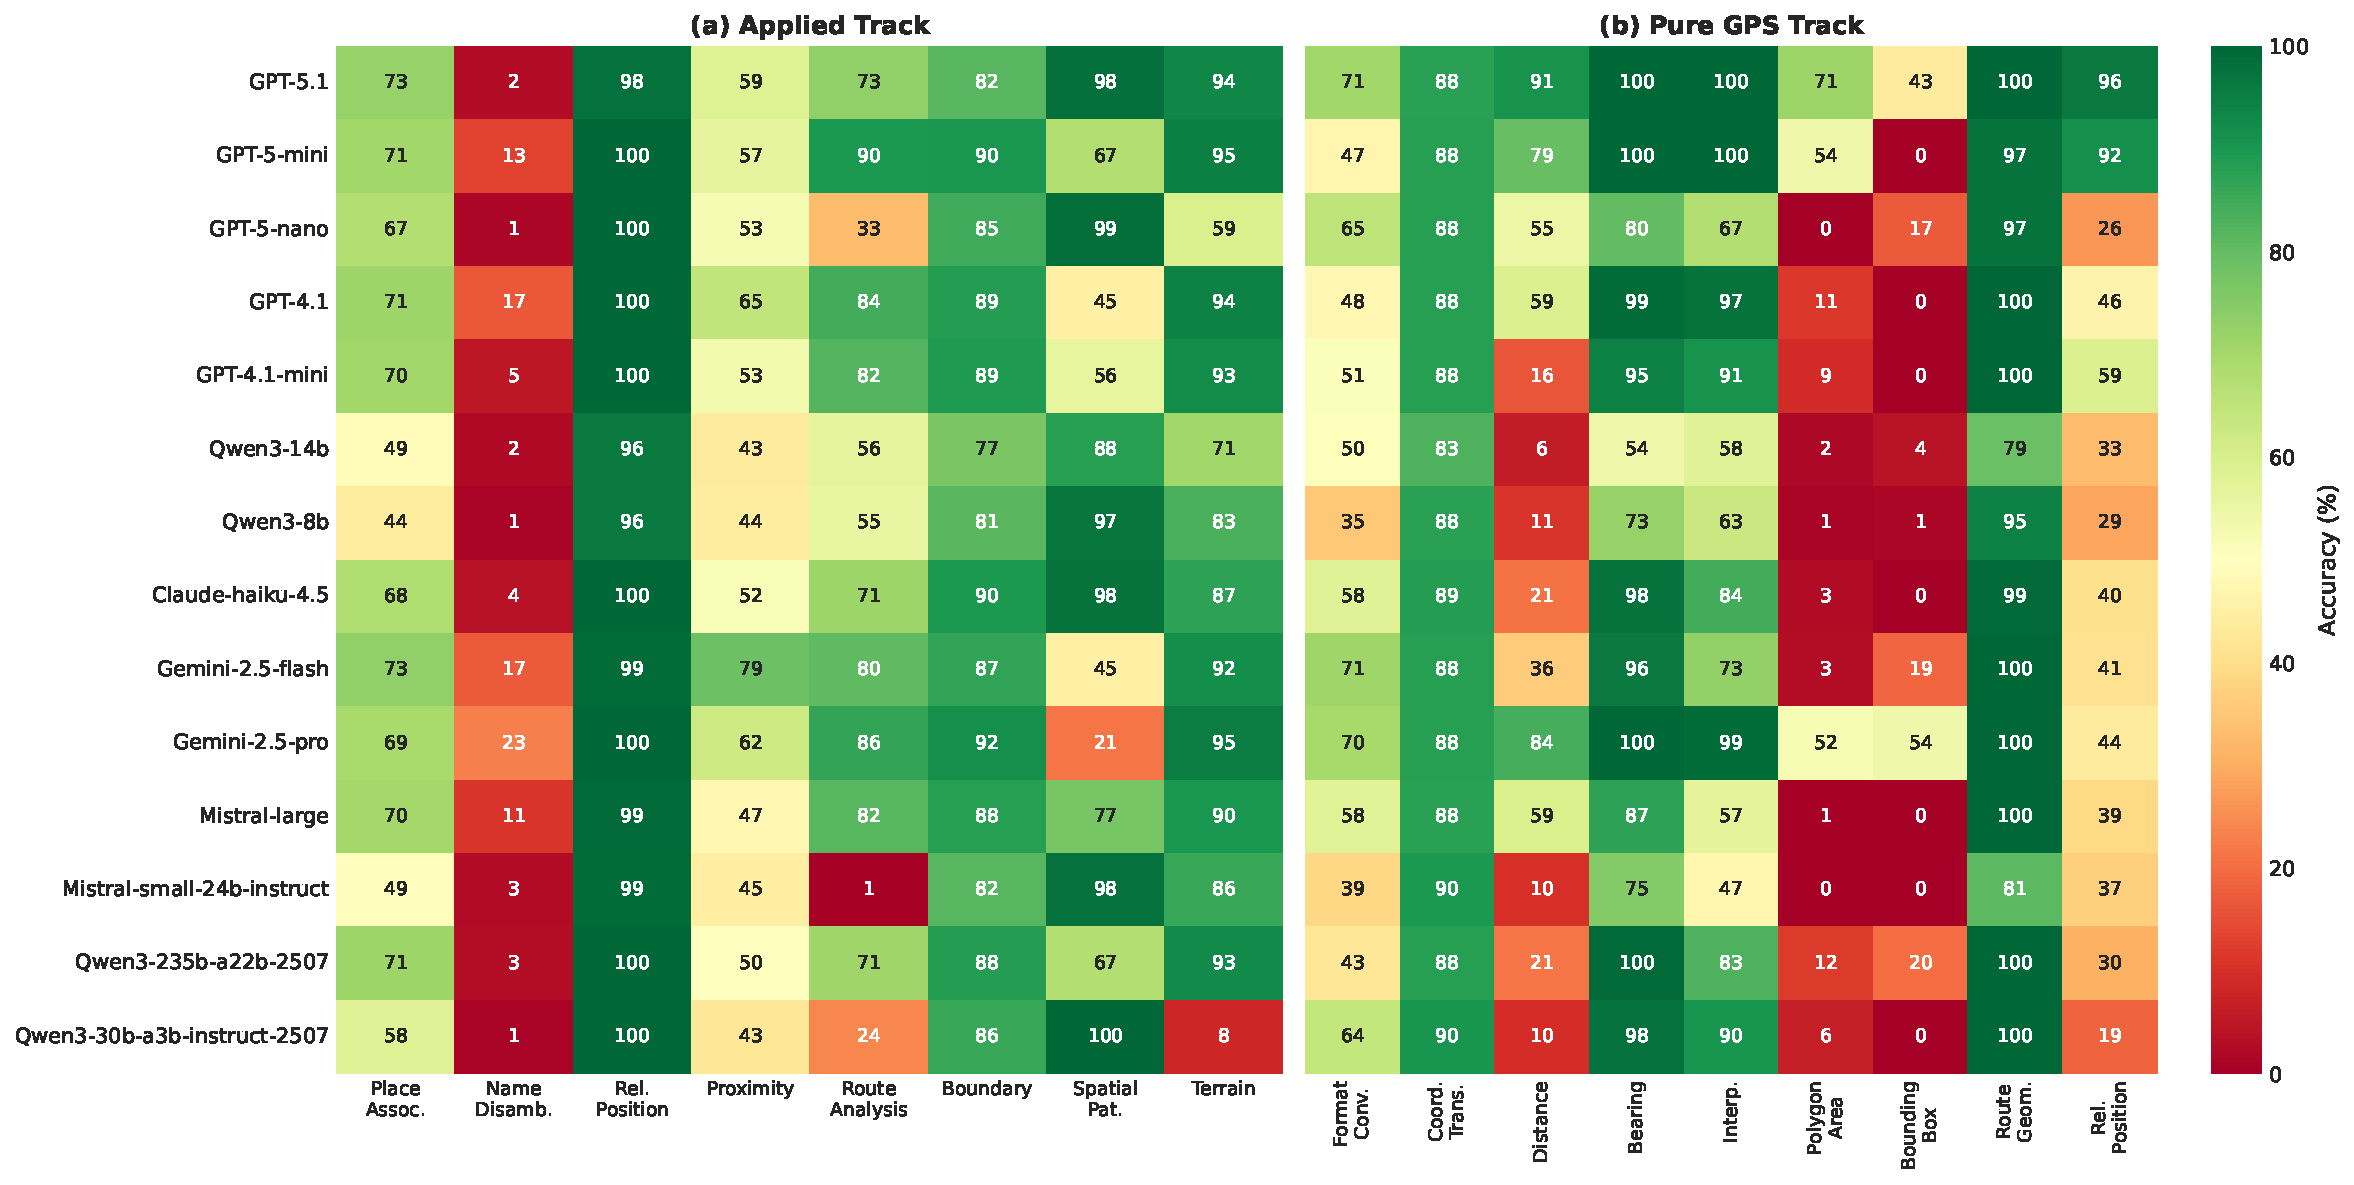
\includegraphics[width=\textwidth]{figures/per_task_heatmap_combined.pdf}
\caption{Per-task accuracy (\%) across 14 LLMs. (a) Applied Track tasks requiring world knowledge integration. (b) Pure GPS Track tasks requiring geometric computation. Green indicates high accuracy, red indicates low accuracy.}
\label{fig:heatmap_detailed}
\end{figure*}

\begin{table*}[htbp]
\centering
\caption{Per-task accuracy (\%) for Applied Track. Bold indicates best per task.}
\label{tab:per_task_applied}
\small
\begin{tabular}{lcccccccc}
\toprule
\textbf{Model} & \textbf{Name} & \textbf{Route} & \textbf{Spatial} & \textbf{Bound.} & \textbf{Terrain} & \textbf{Prox.} & \textbf{Rel. Pos.} & \textbf{Place} \\
\midrule
GPT-5.1 & 97.7 & 81.7 & 93.7 & 98.1 & \textbf{72.6} & 73.3 & 58.5 & 2.5 \\
GPT-5-mini & \textbf{100.0} & 90.1 & 95.2 & 67.4 & 70.6 & \textbf{89.6} & 56.6 & 12.9 \\
GPT-5-nano & 99.9 & 84.8 & 59.4 & 98.5 & 67.4 & 33.1 & 52.6 & 1.3 \\
GPT-4.1 & \textbf{100.0} & 88.6 & 94.2 & 45.2 & 71.3 & 84.4 & 64.8 & 16.8 \\
GPT-4.1-mini & \textbf{100.0} & 89.3 & 92.5 & 56.0 & 70.4 & 82.4 & 53.1 & 4.7 \\
\midrule
Gemini-2.5-Pro & 99.9 & \textbf{91.7} & \textbf{95.4} & 21.5 & 69.2 & 86.4 & 62.2 & \textbf{23.0} \\
Gemini-2.5-Flash & 99.4 & 86.9 & 92.1 & 47.7 & 20.7 & 80.5 & \textbf{87.2} & 17.1 \\
\midrule
Claude-Haiku-4.5 & \textbf{100.0} & 89.7 & 87.4 & 97.6 & 68.1 & 71.3 & 51.7 & 3.6 \\
\midrule
Mistral-Large & 99.4 & 87.9 & 90.1 & 77.3 & 70.3 & 81.8 & 47.5 & 10.6 \\
Mistral-Small-24B & 99.1 & 82.0 & 85.9 & 97.8 & 49.3 & 0.6 & 44.8 & 2.6 \\
\midrule
Qwen3-235B & 99.9 & 88.3 & 92.6 & 67.4 & 71.2 & 70.9 & 50.0 & 2.8 \\
Qwen3-30B & 99.7 & 85.7 & 8.1 & \textbf{99.7} & 57.9 & 24.2 & 42.5 & 0.8 \\
Qwen3-14B & 99.5 & 83.2 & 5.3 & 98.2 & 52.4 & 18.6 & 38.2 & 2.2 \\
Qwen3-8B & 98.9 & 80.1 & 3.8 & 96.5 & 48.6 & 12.4 & 35.1 & 1.0 \\
\midrule
\textit{Mean} & \textit{99.5} & \textit{86.4} & \textit{75.4} & \textit{74.5} & \textit{62.8} & \textit{59.3} & \textit{51.8} & \textit{7.3} \\
\textit{Std} & \textit{0.8} & \textit{3.5} & \textit{32.1} & \textit{24.8} & \textit{15.8} & \textit{30.2} & \textit{13.6} & \textit{7.0} \\
\bottomrule
\end{tabular}
\end{table*}

\begin{table*}[htbp]
\centering
\caption{Per-task accuracy (\%) for Pure GPS Track. Bold indicates best per task.}
\label{tab:per_task_pure_gps}
\small
\begin{tabular}{lccccccccc}
\toprule
\textbf{Model} & \textbf{BBox} & \textbf{Format} & \textbf{Dist.} & \textbf{Bearing} & \textbf{Rel. Pos.} & \textbf{Route} & \textbf{Coord.} & \textbf{Interp.} & \textbf{Polygon} \\
\midrule
GPT-5.1 & 99.7 & 87.8 & \textbf{99.9} & \textbf{99.9} & \textbf{70.7} & \textbf{96.3} & \textbf{90.8} & \textbf{71.4} & 43.4 \\
GPT-5-mini & 97.5 & 88.0 & \textbf{99.9} & \textbf{99.8} & 46.6 & 91.8 & 79.4 & 54.1 & 0.0 \\
GPT-5-nano & 97.5 & 88.0 & 80.4 & 67.3 & 65.5 & 26.4 & 54.7 & 0.3 & 17.1 \\
GPT-4.1 & \textbf{100.0} & 88.1 & 99.1 & 97.5 & 47.5 & 46.0 & 59.0 & 11.4 & 0.0 \\
GPT-4.1-mini & 99.9 & 88.1 & 94.8 & 90.9 & 51.0 & 59.0 & 16.3 & 9.1 & 0.0 \\
\midrule
Gemini-2.5-Pro & \textbf{100.0} & 88.1 & \textbf{99.9} & 99.2 & 69.7 & 43.6 & 84.2 & 52.1 & \textbf{53.9} \\
Gemini-2.5-Flash & \textbf{100.0} & 88.0 & 96.3 & 72.7 & \textbf{70.8} & 41.0 & 36.1 & 2.7 & 18.9 \\
\midrule
Claude-Haiku-4.5 & 99.3 & 88.6 & 97.6 & 84.5 & 58.1 & 40.4 & 20.7 & 2.6 & 0.0 \\
\midrule
Mistral-Large & 99.7 & 87.8 & 87.2 & 56.7 & 57.6 & 39.0 & 59.5 & 0.7 & 0.0 \\
Mistral-Small-24B & 81.2 & 89.8 & 75.3 & 47.1 & 38.6 & 37.1 & 9.9 & 0.1 & 0.0 \\
\midrule
Qwen3-235B & 99.7 & 88.1 & 99.5 & 83.0 & 42.5 & 30.5 & 21.3 & 11.9 & 20.1 \\
Qwen3-30B & \textbf{100.0} & \textbf{90.4} & 97.8 & 90.5 & 64.1 & 18.7 & 9.7 & 6.4 & 0.0 \\
Qwen3-14B & 97.2 & 87.3 & 72.5 & 52.3 & 35.8 & 12.4 & 5.2 & 2.1 & 0.0 \\
Qwen3-8B & 95.8 & 86.1 & 68.2 & 45.1 & 32.4 & 8.6 & 3.8 & 0.8 & 0.0 \\
\midrule
\textit{Mean} & \textit{97.6} & \textit{88.3} & \textit{90.6} & \textit{77.6} & \textit{53.6} & \textit{42.2} & \textit{39.3} & \textit{16.1} & \textit{11.0} \\
\textit{Std} & \textit{5.0} & \textit{1.1} & \textit{12.1} & \textit{20.4} & \textit{13.8} & \textit{26.5} & \textit{31.2} & \textit{24.6} & \textit{18.1} \\
\bottomrule
\end{tabular}
\end{table*}

%% =============================================================================
\subsection{Applied vs.\ Pure GPS Gap Analysis}
\label{app:track_gap}

\begin{table}[htbp]
\centering
\caption{Performance gap between Applied and Pure GPS tracks.}
\label{tab:track_gap}
\small
\begin{tabular}{lccc}
\toprule
\textbf{Model} & \textbf{Applied} & \textbf{Pure GPS} & \textbf{Gap} \\
\midrule
GPT-5.1 & 72.0 & 84.4 & $-$12.4 \\
GPT-5-mini & 74.1 & 73.0 & +1.1 \\
GPT-5-nano & 63.5 & 55.2 & +8.2 \\
GPT-4.1 & 73.3 & 60.9 & +12.3 \\
GPT-4.1-mini & 70.5 & 56.6 & +13.9 \\
\midrule
Gemini-2.5-Pro & 71.7 & 76.7 & $-$5.0 \\
Gemini-2.5-Flash & 73.4 & 58.5 & +14.9 \\
\midrule
Claude-Haiku-4.5 & 71.9 & 54.7 & +17.2 \\
\midrule
Mistral-Large & 72.5 & 54.3 & +18.2 \\
Mistral-Small-24B & 59.8 & 42.1 & +17.7 \\
\midrule
Qwen3-235B & 69.8 & 55.2 & +14.6 \\
Qwen3-30B & 53.9 & 53.1 & +0.8 \\
Qwen3-14B & 50.3 & 35.4 & +14.9 \\
Qwen3-8B & 47.1 & 33.3 & +13.8 \\
\bottomrule
\end{tabular}
\end{table}

\paragraph{Overall Gap Distribution.}
Table~\ref{tab:track_gap} reveals that 12 of 14 models score higher on the Applied Track than on the Pure GPS Track, with gaps ranging from +0.8\% (Qwen3-30B) to +18.2\% (Mistral-Large). The two exceptions are GPT-5.1 ($-$12.4\%) and Gemini-2.5-Pro ($-$5.0\%), both flagship reasoning models whose Pure GPS scores surpass their Applied scores. The mean gap across all 14 models is +9.9\%, confirming that world knowledge encoded during pretraining provides a substantial advantage over raw coordinate-level computation for the majority of current LLMs.

\paragraph{Model Family Patterns.}
The \textbf{GPT family} (5 models) leads both tracks, averaging 70.7\% on Applied and 66.0\% on Pure GPS. A clear split emerges within this family: the reasoning models GPT-5.1 and GPT-5-mini show near-balanced or reversed gaps ($-$12.4\% and +1.1\%), while the non-reasoning GPT-4.1 and GPT-4.1-mini exhibit large positive gaps (+12.3\% and +13.9\%). The \textbf{Gemini family} (2 models) mirrors this pattern: Gemini-2.5-Pro (reasoning) achieves a $-$5.0\% gap while Gemini-2.5-Flash shows +14.9\%. The \textbf{Mistral family} (2 models) exhibits the largest average gap (+17.9\%), with both models showing nearly identical gaps (+18.2\% and +17.7\%) despite a 5$\times$ difference in parameter count, suggesting this reflects a training-data characteristic rather than a scale-dependent phenomenon. The \textbf{Qwen family} (4 models) provides the most granular scaling view: overall accuracy increases from 40.2\% (8B) to 62.5\% (235B), with the Applied--Pure GPS gap narrowing for MoE models. Notably, Qwen3-30B (3B active parameters) achieves a near-zero gap of +0.8\%, suggesting MoE architectures may allocate specialized experts to geometric computation.

\paragraph{Reasoning vs.\ Non-Reasoning Models.}
Across families, the three reasoning models above the $y = x$ diagonal in Figure~\ref{fig:scatter} (GPT-5.1, GPT-5-mini, Gemini-2.5-Pro) have a mean gap of $-$5.4\%, while the remaining 11 models average +13.4\%. This 18.8-percentage-point difference suggests that chain-of-thought reasoning is particularly beneficial for multi-step geodetic calculations that require maintaining numerical precision across sequential computation steps.

%% =============================================================================
\subsection{Geographic Granularity Results}
\label{app:granularity_full}

\begin{table}[htbp]
\centering
\caption{Place association accuracy (\%) by geographic granularity level across all 14 models.}
\label{tab:place_assoc_granularity}
\small
\begin{tabular}{lcccc}
\toprule
\textbf{Model} & \textbf{City} & \textbf{Province} & \textbf{Country} & \textbf{Region} \\
\midrule
GPT-5.1 & 12.9 & 61.2 & 81.1 & 0.4 \\
GPT-5-mini & 2.5 & 44.4 & 77.1 & 0.3 \\
GPT-5-nano & 1.3 & 32.2 & 71.9 & 0.2 \\
GPT-4.1 & 16.8 & 61.7 & 85.4 & 1.4 \\
GPT-4.1-mini & 4.7 & 49.1 & 82.1 & 2.4 \\
\midrule
Gemini-2.5-Pro & 23.0 & 72.9 & 96.5 & 40.0 \\
Gemini-2.5-Flash & 17.1 & 69.1 & 91.8 & 13.0 \\
\midrule
Claude-Haiku-4.5 & 3.6 & 48.9 & 86.0 & 38.4 \\
\midrule
Mistral-Large & 10.6 & 60.0 & 91.8 & 1.0 \\
Mistral-Small-24B & 2.6 & 42.9 & 86.1 & 7.0 \\
\midrule
Qwen3-235B & 2.8 & 52.5 & 86.5 & 2.8 \\
Qwen3-30B & 0.8 & 35.2 & 73.2 & 3.5 \\
Qwen3-14B & 2.2 & 29.8 & 63.4 & 0.1 \\
Qwen3-8B & 1.0 & 26.4 & 59.4 & 1.5 \\
\bottomrule
\end{tabular}
\end{table}

%% =============================================================================
\subsection{Coordinate Noise Analysis}
\label{app:noise_analysis}

We test robustness by adding Gaussian noise to coordinates at all granularity levels. This also probes memorization: if models memorized specific coordinate$\rightarrow$place mappings from training data, perturbing coordinates would break these associations. Table~\ref{tab:noise_by_granularity} shows mean accuracy across models at each granularity level and noise magnitude. The lack of degradation at any level, including high-accuracy country identification (80\%), suggests models encode genuine geographic knowledge rather than memorized coordinate strings.

\begin{table}[htbp]
\centering
\caption{Mean accuracy (\%) by noise level and granularity. All levels show stable performance across noise magnitudes, suggesting generalized knowledge rather than memorization.}
\label{tab:noise_by_granularity}
\small
\begin{tabular}{lccc}
\toprule
\textbf{Noise} & \textbf{Country} & \textbf{Province} & \textbf{City} \\
\midrule
Clean & 80.7 & 46.3 & 7.4 \\
10m & 79.1 ($-$1.6) & 51.8 (+5.5) & 5.8 ($-$1.6) \\
50m & 80.1 ($-$0.5) & 52.1 (+5.8) & 9.3 (+1.9) \\
100m & 82.3 (+1.6) & 45.8 ($-$0.5) & 7.1 ($-$0.3) \\
500m & 82.1 (+1.5) & 49.7 (+3.4) & 7.0 ($-$0.5) \\
1km & 81.0 (+0.4) & 48.3 (+2.0) & 7.0 ($-$0.4) \\
\midrule
\textit{Max $|\Delta|$} & \textit{1.6} & \textit{5.8} & \textit{1.9} \\
\bottomrule
\end{tabular}
\end{table}

Table~\ref{tab:place_assoc_noise_results} shows per-model city-level accuracy changes.

\begin{table}[htbp]
\centering
\caption{Place association accuracy change ($\Delta$\%) relative to clean coordinates across all 14 models. Values show difference from clean baseline. Note: no correlation between noise magnitude and $|\Delta|$ (mean $|\Delta|$ = 1.3--2.1\% across all levels).}
\label{tab:place_assoc_noise_results}
\small
\begin{tabular}{lccccc|c}
\toprule
\textbf{Model} & \textbf{Clean (\%)} & \textbf{$\Delta$10m} & \textbf{$\Delta$50m} & \textbf{$\Delta$100m} & \textbf{$\Delta$500m} & \textbf{$\Delta$1km} \\
\midrule
GPT-5.1 & 13.1 & $-$2.2 & +3.7 & $-$2.0 & $-$0.4 & $-$0.5 \\
GPT-5-mini & 1.7 & $-$1.1 & +0.1 & +2.2 & +2.5 & +0.8 \\
GPT-5-nano & 1.1 & $-$1.1 & +1.9 & +0.2 & $-$1.1 & +0.9 \\
GPT-4.1 & 16.0 & $-$2.7 & +5.7 & $-$1.5 & +0.4 & +2.3 \\
GPT-4.1-mini & 5.7 & $-$3.9 & +0.9 & +0.9 & $-$0.9 & $-$2.7 \\
\midrule
Gemini-2.5-Pro & 24.0 & $-$1.0 & +4.9 & $-$3.6 & $-$3.4 & $-$2.7 \\
Gemini-2.5-Flash & 18.9 & $-$0.7 & $-$0.2 & $-$5.0 & $-$0.1 & $-$4.6 \\
\midrule
Claude-Haiku-4.5 & 4.6 & $-$4.0 & +1.5 & $-$0.6 & $-$0.9 & $-$1.5 \\
\midrule
Mistral-Large & 13.1 & $-$4.7 & $-$1.7 & $-$2.0 & $-$4.7 & $-$2.5 \\
Mistral-Small-24B & 1.7 & $-$1.1 & +1.9 & +2.2 & +0.7 & +1.8 \\
\midrule
Qwen3-235B & 2.9 & $-$1.0 & +0.8 & $-$0.2 & +0.8 & $-$0.3 \\
Qwen3-30B & 0.6 & $-$0.6 & +1.2 & +0.7 & $-$0.6 & +0.4 \\
Qwen3-14B & 0.6 & +0.6 & +3.0 & +2.1 & +1.2 & +2.5 \\
Qwen3-8B & 0.0 & +0.6 & +2.4 & +2.6 & +0.0 & +0.5 \\
\midrule
\textit{Mean $|\Delta|$} & -- & \textit{1.8} & \textit{2.1} & \textit{1.8} & \textit{1.3} & \textit{1.7} \\
\bottomrule
\end{tabular}
\end{table}

%% =============================================================================
\subsection{GPS Augmentation Detailed Results}
\label{app:downstream}

\begin{table}[htbp]
\centering
\caption{Effect of GPS augmentation on downstream tasks (\%). Results using GPT-4.1.}
\label{tab:gps_augmentation_downstream}
\small
\begin{tabular}{llcccc}
\toprule
\textbf{Dataset} & \textbf{Category} & \textbf{N} & \textbf{Base} & \textbf{+GPS} & \textbf{$\Delta$} \\
\midrule
\multirow{4}{*}{\shortstack[l]{MapEval\\(100\% geocoded)}}
    & Trip planning & 11 & 90.9 & 100.0 & +9.1 \\
    & POI queries & 51 & 72.5 & 76.5 & +3.9 \\
    & Nearby search & 3 & 66.7 & 100.0 & +33.3 \\
    \cmidrule{2-6}
    & \textit{Overall} & \textit{66} & \textit{75.8} & \textit{81.8} & \textit{+6.1} \\
\midrule
\multirow{5}{*}{\shortstack[l]{Hierarchical\\Spatial}}
    & Hierarchical bias & 10 & 70.0 & 100.0 & +30.0 \\
    & Alignment bias & 4 & 50.0 & 100.0 & +50.0 \\
    & Proximity bias & 4 & 0.0 & 0.0 & 0.0 \\
    & Rotation bias & 4 & 0.0 & 0.0 & 0.0 \\
    \cmidrule{2-6}
    & \textit{Overall} & \textit{22} & \textit{40.9} & \textit{63.6} & \textit{+22.7} \\
\bottomrule
\end{tabular}
\end{table}

%% =============================================================================
\subsection{Finetuning Analysis}
\label{app:finetuning}

We finetune Qwen3-30B on GPSBench training data and compare against zero-shot performance. Table~\ref{tab:finetuning_overall} shows overall results by track.

\begin{table}[htbp]
\centering
\caption{Overall finetuning results on Qwen3-30B.}
\label{tab:finetuning_overall}
\small
\begin{tabular}{lccc}
\toprule
\textbf{Track} & \textbf{Zero-shot} & \textbf{Finetuned} & \textbf{$\Delta$} \\
\midrule
Applied & 52.3\% & 50.7\% & $-$1.6\% \\
Pure GPS & 53.1\% & 57.4\% & +4.3\% \\
\midrule
\textit{Combined} & \textit{52.7\%} & \textit{54.1\%} & \textit{+1.5\%} \\
\bottomrule
\end{tabular}
\end{table}

Table~\ref{tab:finetuning_per_task} provides per-task breakdown, revealing the divergent effects of finetuning on geometric vs.\ world-knowledge tasks.

\begin{table}[htbp]
\centering
\caption{Per-task finetuning comparison on Qwen3-30B (\%). Green: improvement ($>$5\%), red: degradation ($<$$-$5\%).}
\label{tab:finetuning_per_task}
\small
\begin{tabular}{lccc}
\toprule
\textbf{Task} & \textbf{Zero-shot} & \textbf{Finetuned} & \textbf{$\Delta$} \\
\midrule
\multicolumn{4}{c}{\textit{Applied Track}} \\
\midrule
Place Association & 0.8 & 1.7 & +0.9 \\
Name Disambiguation & 99.7 & 82.6 & \textcolor{red}{$-$17.1} \\
Relative Position & 42.5 & 22.9 & \textcolor{red}{$-$19.6} \\
Proximity & 24.2 & 15.4 & \textcolor{red}{$-$8.8} \\
Route Analysis & 85.7 & 89.9 & +4.2 \\
Boundary Analysis & 99.7 & 74.5 & \textcolor{red}{$-$25.2} \\
Spatial Patterns & 8.1 & 64.6 & \textcolor{green!60!black}{+56.5} \\
Terrain & 57.9 & 53.9 & $-$4.0 \\
\midrule
\textit{Applied Overall} & \textit{52.3} & \textit{50.7} & \textit{$-$1.6} \\
\midrule
\multicolumn{4}{c}{\textit{Pure GPS Track}} \\
\midrule
Format Conversion & 90.4 & 90.9 & +0.5 \\
Coord.\ Transform & 9.7 & 6.6 & $-$3.1 \\
Distance & 97.8 & 94.2 & $-$3.6 \\
Bearing & 90.5 & 78.2 & \textcolor{red}{$-$12.3} \\
Interpolation & 6.4 & 25.3 & \textcolor{green!60!black}{+18.9} \\
Polygon Area & 0.0 & 25.9 & \textcolor{green!60!black}{+25.9} \\
Bounding Box & 100.0 & 99.9 & $-$0.1 \\
Route Geometry & 18.7 & 31.1 & \textcolor{green!60!black}{+12.4} \\
Relative Position & 64.1 & 64.1 & 0.0 \\
\midrule
\textit{Pure GPS Overall} & \textit{53.1} & \textit{57.4} & \textit{+4.3} \\
\bottomrule
\end{tabular}
\end{table}

%% =============================================================================
\subsection{Regional Performance Breakdown}
\label{app:regional_performance}

We analyze regional performance across all GPSBench tasks by extracting location information from coordinates, country codes, and prompt text (Figure~\ref{fig:regional_all_tasks_comprehensive}). The results reveal that \textit{geographic bias is task-specific, not universal}.

\paragraph{Task-Specific Patterns.}
Place Association shows the strongest regional bias: North America (14.7\%) and Western Europe (11.0\%) outperform South Asia (2.6\%) and East Asia (3.8\%) by 4--6$\times$. This reflects sparse coordinate-to-city mappings in training data for non-Western regions. In contrast, most Pure GPS computation tasks show minimal regional variation: Distance (74.6--83.3\%), Bounding Box (95.2--98.5\%), and Format Conversion (97.4--100\%) are nearly uniform across subregions, confirming that geometric computation is region-agnostic. Name Disambiguation shows no bias (97.1--100\%), indicating this task is ``solved'' regardless of location. The comprehensive analysis confirms that geographic bias stems primarily from knowledge gaps rather than computational limitations.

\begin{figure*}[htbp]
\centering
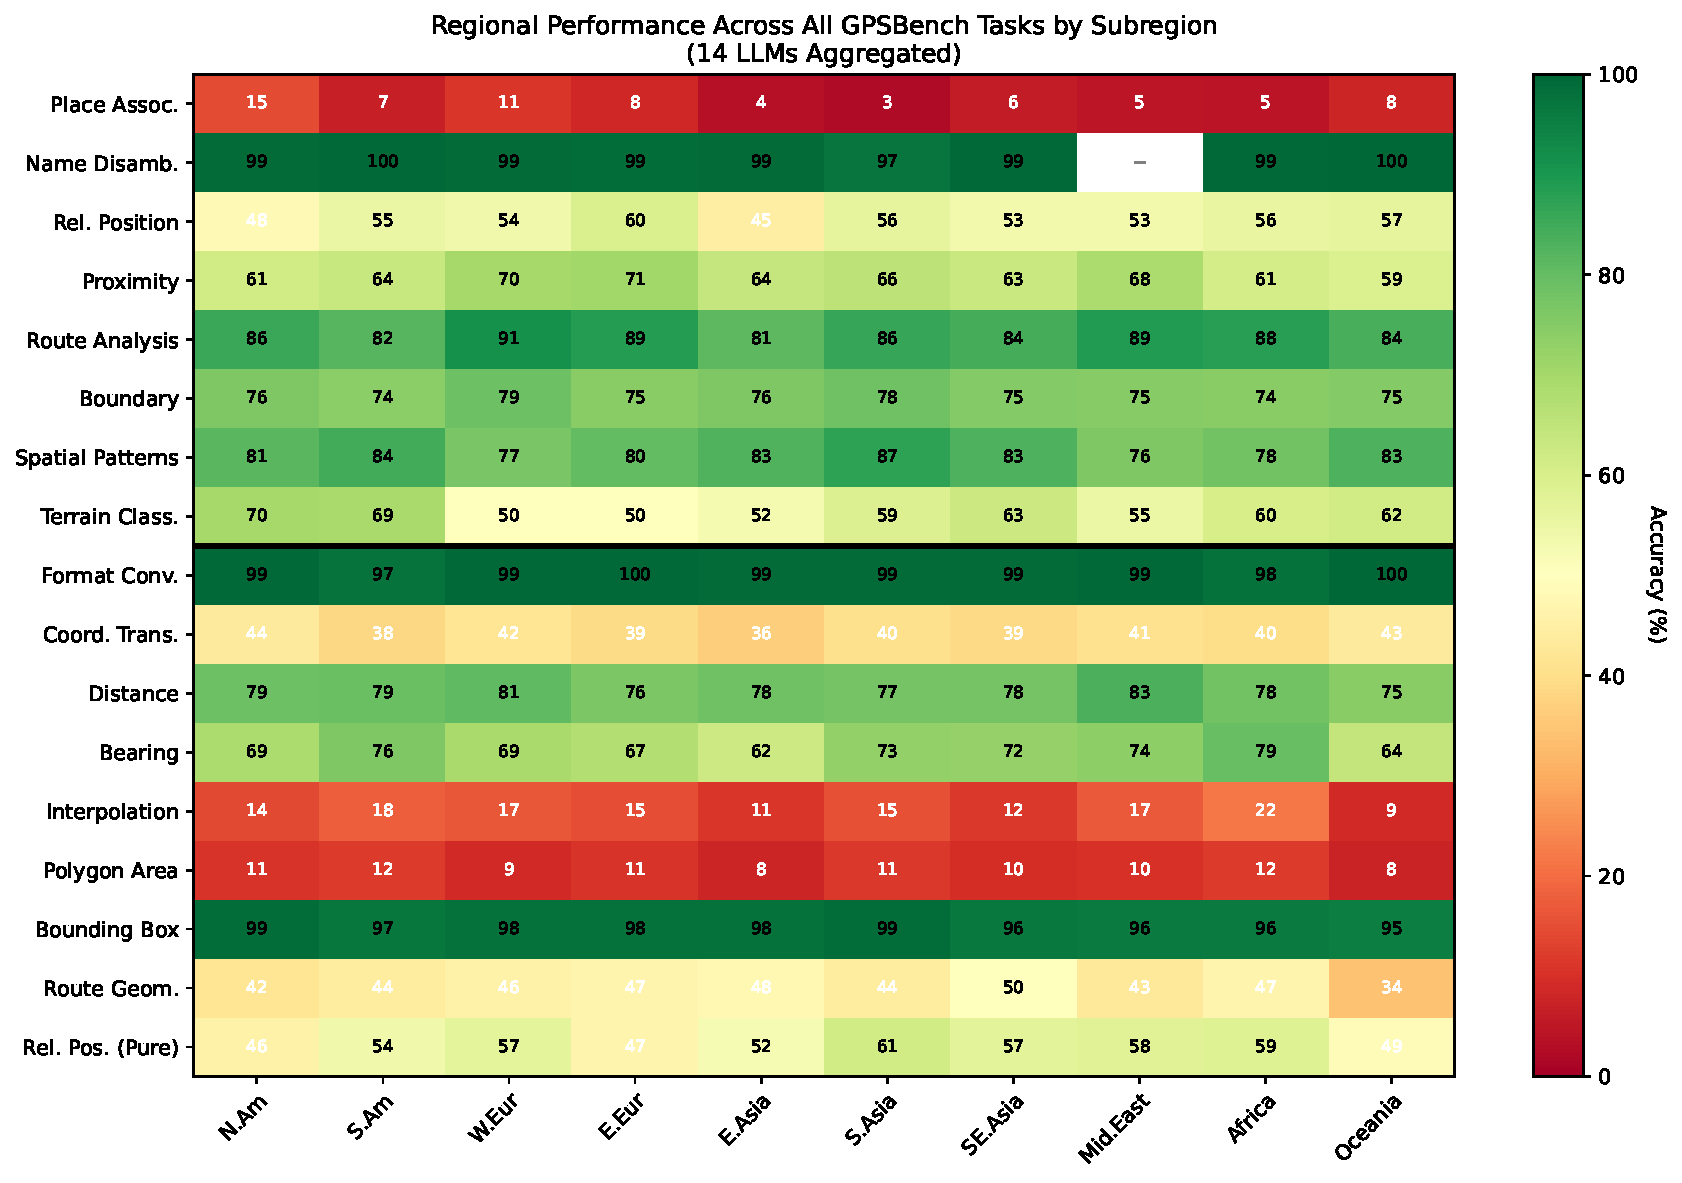
\includegraphics[width=\textwidth]{figures/regional_all_tasks_comprehensive.pdf}
\caption{Regional performance across all GPSBench tasks by subregion (14 LLMs aggregated). Applied Track tasks (top) show varying degrees of geographic bias, with Place Association exhibiting the strongest disparity. Pure GPS Track tasks (bottom) show minimal regional variation, confirming that geometric computation is largely region-agnostic.}
\label{fig:regional_all_tasks_comprehensive}
\end{figure*}

\begin{table*}[htbp]
\centering
\caption{Accuracy (\%) by subregion across all GPSBench tasks (14 LLMs aggregated). Tasks are grouped by track. Bold indicates highest accuracy per task; -- indicates insufficient data.}
\label{tab:regional_all_tasks_comprehensive}
\small
\begin{tabular}{lcccccccccc}
\toprule
\textbf{Task} & \textbf{N.Am} & \textbf{S.Am} & \textbf{W.Eur} & \textbf{E.Eur} & \textbf{E.Asia} & \textbf{S.Asia} & \textbf{SE.Asia} & \textbf{M.East} & \textbf{Africa} & \textbf{Oceania} \\
\midrule
\multicolumn{11}{l}{\textit{Applied Track}} \\
Place Assoc. & \textbf{14.7} & 6.7 & 11.0 & 8.3 & 3.8 & 2.6 & 5.9 & 5.0 & 4.5 & 8.0 \\
Name Disamb. & 99.1 & 99.5 & 99.1 & 98.8 & 98.8 & 97.1 & 99.3 & -- & 99.4 & \textbf{100.0} \\
Rel. Position & 48.1 & 55.4 & 53.7 & \textbf{59.7} & 44.6 & 56.5 & 53.1 & 53.4 & 55.8 & 56.5 \\
Proximity & 61.4 & 63.6 & 69.6 & \textbf{70.6} & 63.7 & 65.6 & 63.2 & 68.5 & 60.8 & 59.2 \\
Route Analysis & 85.8 & 81.8 & \textbf{91.4} & 88.6 & 80.9 & 86.2 & 84.3 & 88.8 & 88.2 & 84.0 \\
Boundary & 75.9 & 73.8 & \textbf{78.6} & 74.6 & 76.0 & 78.3 & 75.1 & 74.7 & 74.3 & 75.1 \\
Spatial Patterns & 81.4 & 84.4 & 76.9 & 80.4 & 82.6 & \textbf{87.1} & 82.9 & 76.1 & 78.0 & 83.1 \\
Terrain Class. & \textbf{69.8} & 69.3 & 50.3 & 50.0 & 52.4 & 58.8 & 62.6 & 55.0 & 60.4 & 61.6 \\
\midrule
\multicolumn{11}{l}{\textit{Pure GPS Track}} \\
Format Conv. & 99.5 & 97.4 & 99.3 & 99.5 & 98.9 & 99.1 & 98.9 & 99.5 & 97.8 & \textbf{100.0} \\
Coord. Trans. & \textbf{43.7} & 38.4 & 41.8 & 39.3 & 36.4 & 40.3 & 38.8 & 40.9 & 39.5 & 43.5 \\
Distance & 78.9 & 79.0 & 80.6 & 76.4 & 78.2 & 77.4 & 77.7 & \textbf{83.3} & 78.1 & 74.6 \\
Bearing & 68.6 & 75.8 & 69.2 & 67.4 & 62.3 & 72.7 & 72.4 & 73.7 & \textbf{79.4} & 64.4 \\
Interpolation & 14.2 & 17.9 & 16.7 & 14.9 & 11.2 & 15.4 & 11.6 & 17.1 & \textbf{21.7} & 8.6 \\
Polygon Area & 10.6 & \textbf{12.0} & 8.9 & 10.9 & 7.9 & 11.4 & 9.5 & 10.2 & 11.9 & 7.8 \\
Bounding Box & \textbf{98.5} & 96.7 & 98.0 & 97.8 & 97.9 & \textbf{98.5} & 96.4 & 96.1 & 95.9 & 95.2 \\
Route Geom. & 41.9 & 43.8 & 46.0 & 46.8 & 47.8 & 43.9 & \textbf{50.0} & 43.3 & 46.7 & 34.1 \\
Rel. Pos. (Pure) & 45.9 & 53.9 & 56.9 & 46.5 & 52.3 & \textbf{61.4} & 57.3 & 57.9 & 58.5 & 48.6 \\
\bottomrule
\end{tabular}
\end{table*}

%% =============================================================================
\subsection{Qualitative Error Analysis}
\label{app:error_analysis}

We analyze model outputs across tasks to identify systematic error patterns. Table~\ref{tab:error_patterns} summarizes the dominant failure modes for a subset of tasks where clear patterns emerge.

\begin{table}[htbp]
\centering
\caption{Dominant error patterns by task category.}
\label{tab:error_patterns}
\small
\begin{tabular}{p{2.8cm}p{4.7cm}}
\toprule
\textbf{Task} & \textbf{Dominant Error Pattern} \\
\midrule
Place Association & Nearby city substitution \\
Polygon Area & Formula stated but not executed \\
Interpolation & Cumulative numerical errors \\
Coord. Transform & Nonlinear projection arithmetic \\
Bearing/Distance & Computational approximations \\
Spatial Patterns & Heuristic-based reasoning \\
Format Conversion & Precision mismatch \& hemisphere swaps \\
\bottomrule
\end{tabular}
\end{table}

\paragraph{Place Association: Nearby City Substitution.}
Models consistently identify the correct country and province but substitute larger nearby cities for exact locations. For example, given coordinates 10.607°N, 72.979°W (Villanueva, Colombia), GPT-4.1 responds ``Maicao, La Guajira, Colombia'': the correct province but wrong city (Maicao is 50km away). Similarly, coordinates for Emure-Ekiti, Nigeria yield ``Akure, Ondo State, Nigeria'' (the state capital). This pattern confirms that models encode coarse geographic knowledge but lack dense coordinate-to-city mappings:

\begin{quote}
\small
\textbf{Input:} What location is at coordinates 7.436403, 5.459255?\\
\textbf{Ground Truth:} Emure-Ekiti, Nigeria\\
\textbf{GPT-4.1:} ``The coordinates are in Nigeria. Specifically, this point is in the city of Akure, the capital of Ondo State.''\\
\textbf{Analysis:} Correct country and state, but substitutes state capital for actual city.
\end{quote}

\paragraph{Polygon Area: Formula Without Execution.}
Models correctly identify the spherical excess formula but fail to execute the multi-step calculation precisely. Responses typically show abbreviated reasoning (``Approximate calculation yields...'') followed by estimates that deviate significantly from ground truth:

\begin{quote}
\small
\textbf{Input:} Calculate the area of the polygon: Launceston, City of Port Phillip, Hervey Bay, Greenacre (Australia)\\
\textbf{Ground Truth:} 371,518 km\textsuperscript{2}\\
\textbf{GPT-4.1:} ``Use the spherical excess formula for a quadrilateral: Area $\approx$ E $\times$ R$^2$... Approximate calculation yields: FINAL ANSWER: 2,200,000 km\textsuperscript{2}''\\
\textbf{Analysis:} States correct method but estimate is 5.9$\times$ too large.
\end{quote}

\paragraph{Interpolation: Cumulative Numerical Errors.}
Models correctly apply the spherical linear interpolation (slerp) algorithm conceptually but accumulate errors through multi-step calculations (coordinate conversion $\rightarrow$ Cartesian transformation $\rightarrow$ angle computation $\rightarrow$ weighting $\rightarrow$ interpolation $\rightarrow$ normalization $\rightarrow$ back-conversion). With tight tolerance (0.01°), even small intermediate errors compound:

\begin{quote}
\small
\textbf{Input:} Find the point 0.5 of the way from West Englewood (41.778°N, 87.667°W) to Achaguas (7.779°N, 68.224°W)\\
\textbf{Ground Truth:} 25.089°N, 76.560°W\\
\textbf{GPT-4.1:} 25.104°N, 76.484°W\\
\textbf{Analysis:} Latitude error: 0.015° ($>$ 0.01° tolerance), longitude error: 0.076°. Close but fails due to accumulated rounding in intermediate steps.
\end{quote}

\paragraph{Bearing Computation: High Success Rate.}
Bearing computation achieves high accuracy (up to 97.7\% for GPT-4.1) because it requires fewer computational steps than interpolation and has generous tolerance ($\pm$5°). The few failures occur on long-distance, cross-hemisphere routes where the great-circle path crosses the antimeridian:

\begin{quote}
\small
\textbf{Input:} Calculate bearing from Tacloban, Philippines (11.24°N, 125.00°E) to Cimarron Hills, USA (38.86°N, 104.70°W)\\
\textbf{Ground Truth:} 39.77° (NE)\\
\textbf{GPT-4.1:} [Explains formula but calculation incomplete]\\
\textbf{Analysis:} Cross-Pacific routes require careful handling of longitude wrapping; model's intermediate steps are correct but final computation not completed.
\end{quote}

\paragraph{Spatial Patterns: Heuristic-Based Reasoning.}
When the geographic outlier is obvious (e.g., one city on a different continent), models succeed reliably. Errors occur when city names are ambiguous or when models apply simple geographic heuristics instead of computing centroid distances:

\begin{quote}
\small
\textbf{Input:} Which location is the geographic outlier: Hunts Cross, Atkarsk, Moskovskiy, Challans, Rye?\\
\textbf{Ground Truth:} Rye (Australia, 5,657 km from centroid)\\
\textbf{GPT-4.1:} ``Rye is a town in East Sussex, England... Atkarsk is the farthest east and most distant from the cluster of Western European locations. FINAL ANSWER: Atkarsk''\\
\textbf{Analysis:} Model incorrectly identifies Rye as the English town rather than Rye, Victoria, Australia. Uses ``farthest east'' heuristic instead of computing centroid distances, selecting Atkarsk (Russia, 3,068 km) over the true outlier.
\end{quote}

\paragraph{Coordinate System Transformation: Nonlinear Projection Arithmetic.}
Error rates track projection complexity. UTM (Transverse Mercator) fails far more often than Web Mercator, and within Web Mercator, the linear $x$-formula ($x = R\lambda$) is usually correct while the nonlinear $y$-formula involving \texttt{tan} and \texttt{ln} accounts for nearly all errors. This suggests models can handle linear arithmetic but struggle with chains of transcendental functions. Southern-hemisphere UTM is especially error-prone, as models sometimes truncate the 10-million-meter false northing offset:

\begin{quote}
\small
\textbf{Input:} Convert WGS84 coordinates for Ngong, Kenya (-1.3527°, 36.6699°) to UTM Zone 37S.\\
\textbf{Ground Truth:} Easting: 240,718 m, Northing: 9,850,361 m\\
\textbf{GPT-4.1:} Easting: 266,222 m, Northing: 985,045 m\\
\textbf{Analysis:} Easting is off by 25 km, and Northing drops a digit (985K instead of 9.85M), omitting the southern-hemisphere false northing.
\end{quote}

\paragraph{Distance and Bearing: Computational Approximations.}
While models correctly identify formulas (Haversine, forward azimuth), multi-step calculations accumulate numerical errors. Distance errors typically range 5--15\% from ground truth:

\begin{quote}
\small
\textbf{Input:} Calculate the distance from Kurseong, India to General Villegas, Argentina.\\
\textbf{Ground Truth:} 17,143 km\\
\textbf{GPT-4.1:} 15,857 km\\
\textbf{Analysis:} Correct Haversine approach but 7.5\% underestimate, likely from intermediate rounding in the angular distance calculation.
\end{quote}

\paragraph{Format Conversion: Precision Mismatch and Hemisphere Swaps.}
Most format conversion errors fall into two categories. The majority are \textit{precision mismatches}: the model outputs correct values but with extra or missing decimal places (e.g., ``30.43\arcsec'' vs.\ the expected ``30.4\arcsec''). A smaller class involves \textit{hemisphere label swaps}, where the N/S and E/W indicators are transposed between latitude and longitude:

\begin{quote}
\small
\textbf{Input:} Convert 2.408500°, 42.977100° to DMS format.\\
\textbf{Ground Truth:} 2°24'30.6"N, 42°58'37.6"E\\
\textbf{GPT-4.1:} 2°24'30.6"E, 42°58'37.6"N\\
\textbf{Analysis:} Numerical conversion is exact, but N and E labels are swapped, producing an invalid coordinate.
\end{quote}

\paragraph{Summary.}
Error analysis reveals three distinct failure causes: (1) \textbf{knowledge gaps}, where models lack dense coordinate-to-city mappings and default to nearby prominent cities; (2) \textbf{nonlinear arithmetic}, where models state correct geodetic formulas but fail to evaluate transcendental functions (sin, tan, ln) needed for projections and spherical geometry; and (3) \textbf{heuristic reasoning}, where models apply geographic shortcuts (e.g., ``farthest east'') instead of computing distances. Scaling may address (1), but (2) points to a limitation of autoregressive generation for precise numerical computation.
